\documentclass[10pt]{beamer}

% Pakiety językowe i kodowanie
\usepackage[utf8]{inputenc}
\usepackage[T1]{fontenc}
\usepackage[polish]{babel}
\usepackage{graphicx}
\usepackage{booktabs}
\usepackage{amsmath}

\usetheme{Madrid}
\usecolortheme{whale}

\title[\textbf{Funkcje Interpolacji Fraktalnych}]{Funkcje Interpolacji Fraktalnych}
\subtitle{Analiza funkcji Weierstrassa, krzywych Peano i FIF}
\author[R. Filarecki, E. Mołczan]{Rafał Filarecki \and Ernest Mołczan}
\date{\today}

\begin{document}

\begin{frame}
    \titlepage
\end{frame}

\begin{frame}{Cel i zakres pracy}
    \begin{itemize}
        \item \textbf{Główny cel:} Analiza trzech klas obiektów fraktalnych i badanie ich wymiaru fraktalnego metodą numeryczną.
        \item \textbf{Metodologia:} Wykorzystanie algorytmu \textit{box-counting} zaimplementowanego w języku Python.
        \item \textbf{Badane obiekty:}
        \begin{enumerate}
            \item Funkcja Weierstrassa (ciągła, nigdzie nieróżniczkowalna).
            \item Krzywe wypełniające przestrzeń (Hilbert, Peano, Smok).
            \item Fraktalne Funkcje Interpolacyjne (FIF).
        \end{enumerate}
        \item \textbf{Kluczowy problem:} Weryfikacja dokładności metod numerycznych względem wartości teoretycznych.
    \end{itemize}
\end{frame}

\begin{frame}{Weryfikacja metody box-counting}
    \begin{columns}
        \begin{column}{0.5\textwidth}
            \textbf{Obiekty podstawowe:}
            \begin{itemize}
                \item Linia prosta ($D=1$): błąd $\sim 1\%$.
                \item Kwadrat ($D=2$): błąd $\sim 6\%$.
                \item Okrąg ($D=1$): błąd $\sim 7.5\%$.
            \end{itemize}
            \vspace{0.5cm}
            \textbf{Fraktale klasyczne:}
            \begin{itemize}
                \item Trójkąt Sierpińskiego: $D_{num} = 1.5795$ (błąd $< 0.4\%$).
                \item Dywan Sierpińskiego: $D_{num} = 1.8654$ (błąd $\sim1.4\%$).
            \end{itemize}
        \end{column}
            \begin{column}{0.5\textwidth}
                \begin{figure}
                    \centering
                    
\includegraphics[width=\textwidth]{box_counting_verification.png}
                    \caption{Weryfikacja na figurach płaskich}
                \end{figure}
            \end{column}
    \end{columns}
\end{frame}

\begin{frame}{Funkcja Weierstrassa}
    \begin{itemize}
        \item \textbf{Definicja:} $W(x) = \sum_{n=0}^{\infty} a^n \cos(b^n \pi x)$
        \item \textbf{Własność:} Funkcja ciągła, ale nigdzie nieróżniczkowalna dla $ab > 1$.
        \item \textbf{Wymiar teoretyczny:} $D = 2 + \frac{\log a}{\log b}$
    \end{itemize}
    \begin{figure}
        \centering
        
\includegraphics[width=\textwidth]{weierstrass_box_counting.png}
        \caption{Wykres dla $a=0.5, b=3$}
    \end{figure}
\end{frame}

% Slajd 5: Wpływ parametrów a i b na wymiar
\begin{frame}{Wpływ parametrów $a$ i $b$ na wymiar}
    \begin{itemize}
        \item \textbf{Parametr $a$ (tłumienie):} Wzrost $a$ drastycznie zwiększa "szorstkość" i wymiar fraktalny. Błąd numeryczny rośnie od $3\%$ do $25\%$.
        \item \textbf{Parametr $b$ (częstotliwość):} Zwiększanie $b$ przesuwa detale fraktalne na mniejsze skale.
    \end{itemize}
    \begin{columns}
        \begin{column}{0.5\textwidth}
            \centering
            
\includegraphics[width=\textwidth]{weierstrass_dimension_vs_a.png}
        \end{column}
        \begin{column}{0.5\textwidth}
            \centering
            
\includegraphics[width=\textwidth]{weierstrass_dimension_vs_b.png}
        \end{column}
    \end{columns}
    \begin{alertblock}{Wniosek}
        Metoda box-counting systematycznie niedoszacowuje wymiaru przy wysokiej złożoności (saturacja numeryczna).
    \end{alertblock}
\end{frame}

% Slajd 6: Krzywe wypełniające przestrzeń
\begin{frame}{Krzywe wypełniające przestrzeń}
    \begin{itemize}
        \item \textbf{Paradoks:} Krzywa (obiekt 1D) przechodzi przez każdy punkt kwadratu (obiekt 2D).
        \item \textbf{Analizowane krzywe:} Hilberta, Peano, Smoka.
    \end{itemize}
    \begin{figure}
    \centering
    
\includegraphics[width=\textwidth]{curves_comparison.png}
    \caption{Porównanie badanych konstrukcji}
    \end{figure}
\end{frame}

\begin{frame}{Analiza wymiaru krzywych Peano i Hilberta}
    \begin{columns}
        \begin{column}{0.45\textwidth}
            \begin{itemize}
                \item Wraz ze wzrostem rzędu iteracji, wymiar numeryczny zbiega do $D=2$.
                \item \textbf{Krzywa Peano:} Najszybsza zbieżność ($D \approx 1.96$ już w 5. rzędzie).
                \item \textbf{Krzywa Smoka:} Wykazuje saturację na poziomie $D \approx 1.77$.
            \end{itemize}
        \end{column}
        \begin{column}{0.55\textwidth}
        \begin{figure}
            \centering
            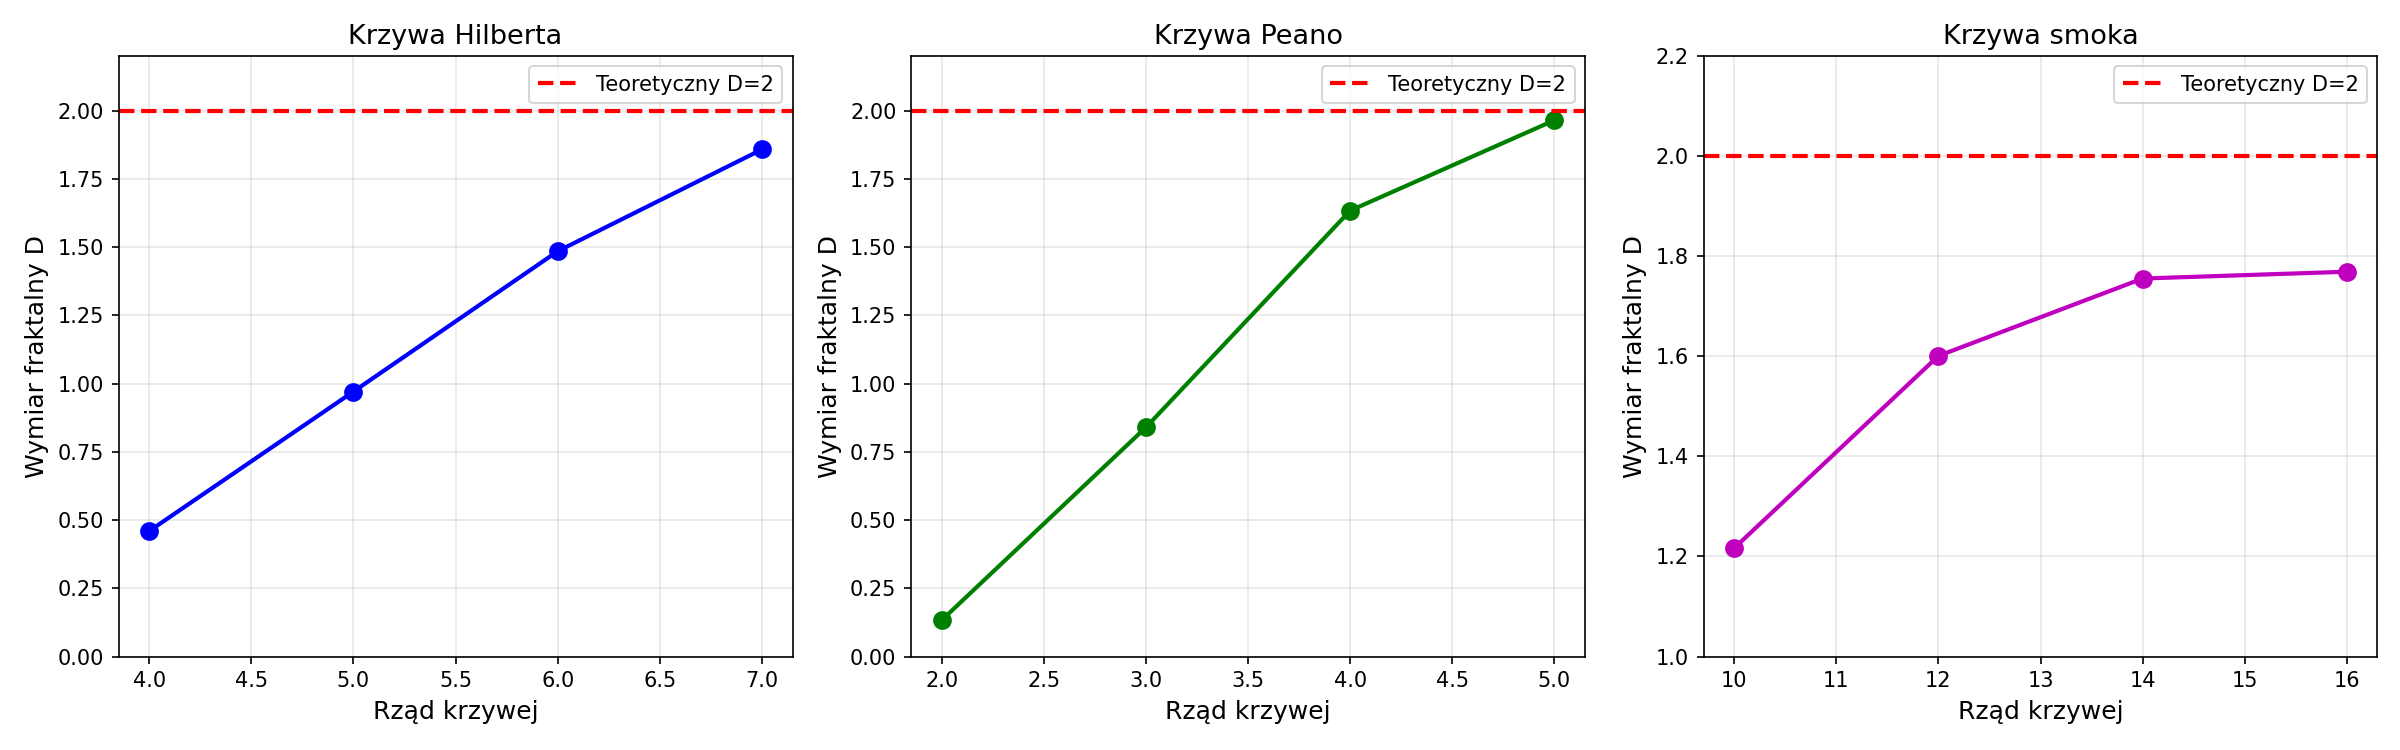
\includegraphics[width=\textwidth]{space_filling_dimensions_vs_order.png}
            \caption{Trend zbieżności wymiaru}
        \end{figure}
            
        \end{column}
    \end{columns}
\end{frame}

\begin{frame}{Fraktalne Funkcje Interpolacyjne (FIF)}
    \begin{itemize}
        \item \textbf{Zastosowanie:} Interpolacja danych o nieregularnej, "naturalnej" strukturze.
        \item \textbf{Parametr $d$:} Kontroluje pionowe skalowanie i szorstkość atraktora.
    \end{itemize}
    \begin{figure}
        \centering
        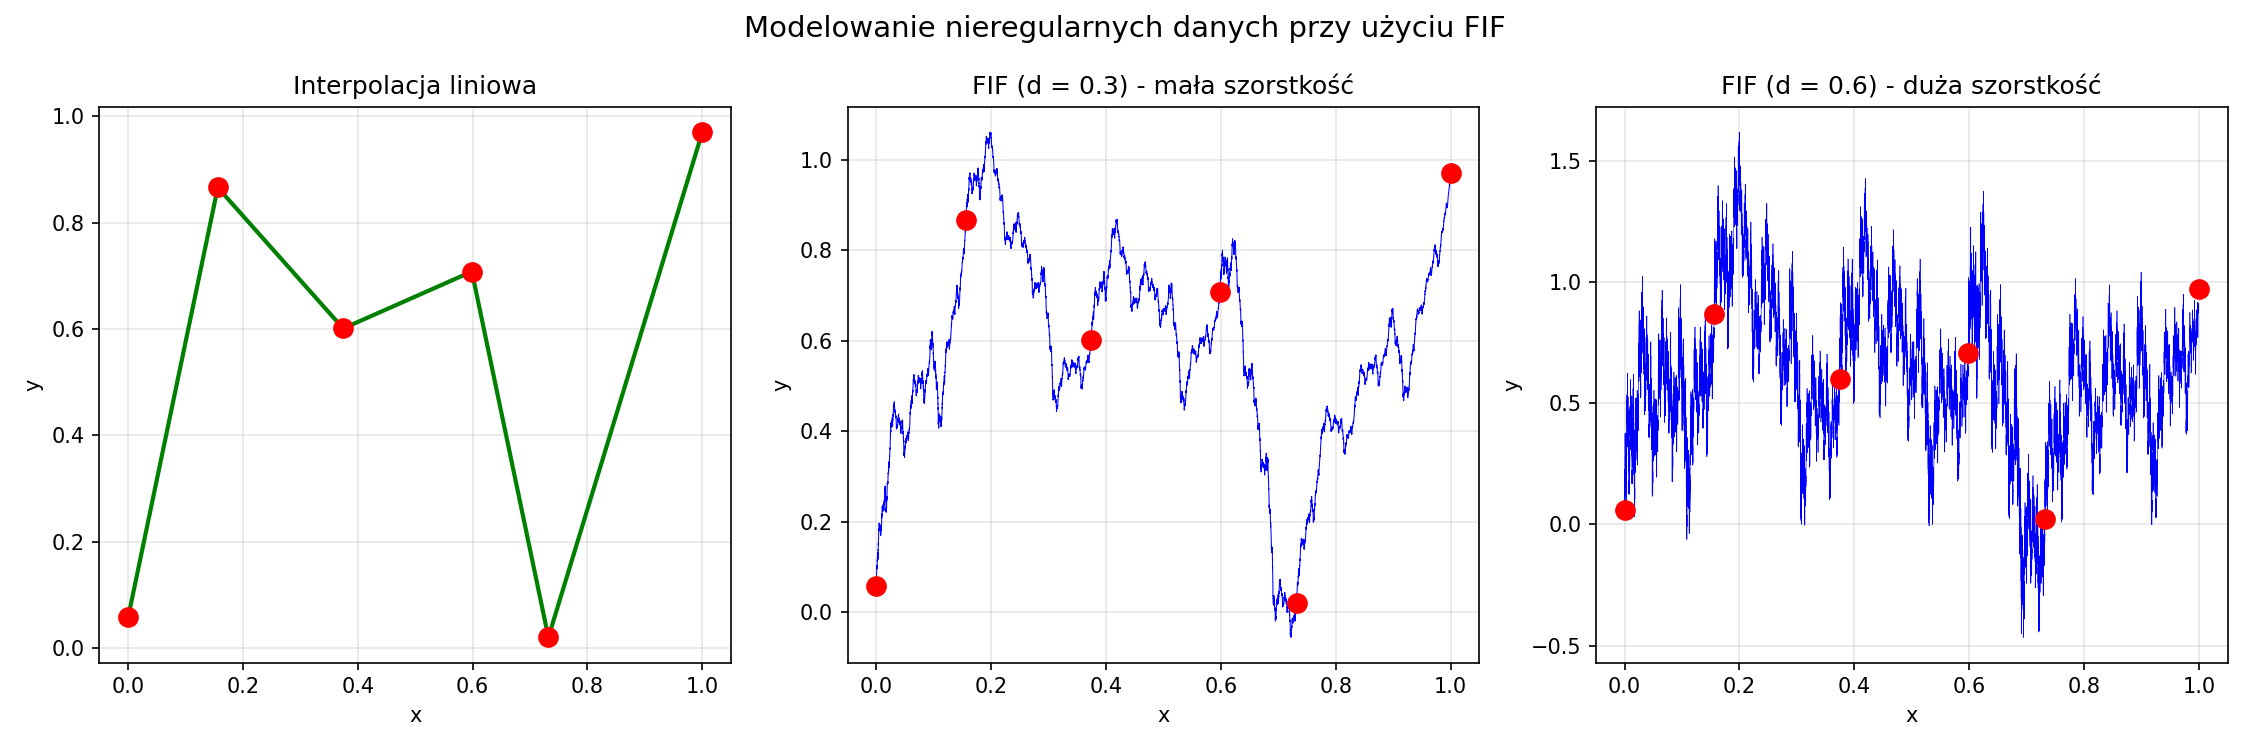
\includegraphics[width=0.8\linewidth]{fif_application.png}
        \caption{Modelowanie danych przy różnych wartościach $d$}
        \label{fig:placeholder}
    \end{figure}
\end{frame}

\begin{frame}{Dlaczego box-counting zawodzi dla FIF?}
    \begin{columns}
        \begin{column}{0.5\textwidth}
            \centering
            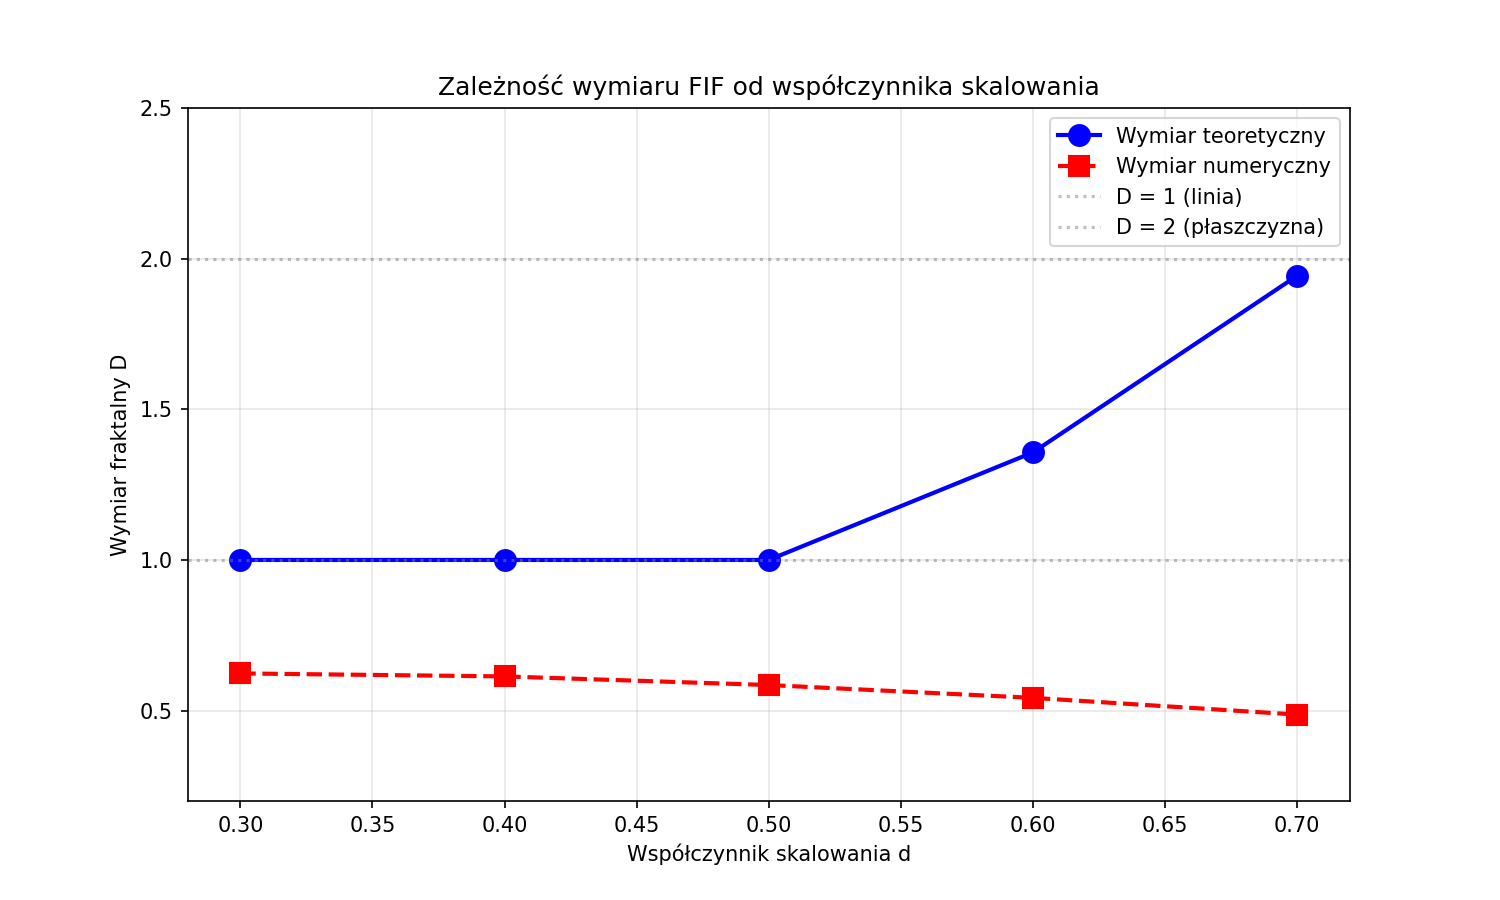
\includegraphics[width=\textwidth]{fif_dimension_vs_d.png}
        \end{column}
        \begin{column}{0.5\textwidth}
            \textbf{Przyczyny błędu:}
            \begin{enumerate}
                \item \textbf{Skończona rozdzielczość:} Gwałtowne oscylacje są mniejsze niż krok dyskretyzacji $x$.
                \item \textbf{Zjawisko "rozpadu":} Algorytm widzi chmurę punktów zamiast linii, co zaniża wymiar.
                \item \textbf{Skala pionowa:} Przy $d \to 1$ amplituda oscylacji przekracza zakresy skalowania pudełek.
            \end{enumerate}
        \end{column}
    \end{columns}
\end{frame}

\begin{frame}{Podsumowanie i wnioski}
    \begin{itemize}
        \item Metoda \textit{box-counting} jest skutecznym narzędziem do badania samopodobieństwa, ale posiada granice stosowalności.
        \item \textbf{Główne problemy numeryczne:}
        \begin{itemize}
            \item Skończona liczba punktów.
            \item Stały zakres rozmiarów pudełek $\varepsilon$.
            \item Saturacja przy wysokiej "szorstkości" funkcji.
        \end{itemize}
    \end{itemize}
\end{frame}

\end{document}